\documentclass[]{beamer}
%\documentclass{article}
%\usepackage{beamerarticle}

\mode<presentation>
{
  \usetheme{Warsaw}
  % or ...

  \setbeamercovered{transparent}
  % or whatever (possibly just delete it)
}


\usepackage[english]{babel}
% or whatever

\usepackage[utf8]{inputenc}
% or whatever

\usepackage{times}
\usepackage[T1]{fontenc}

%%%%%%%%%%%%%%%%%%%%%%%%%%%%%%%%%%
%%                         PACKAGES                      %%
%%%%%%%%%%%%%%%%%%%%%%%%%%%%%%%%%%
\usepackage{hyperref,ctable}
\usepackage{graphicx}
\usepackage{tikz}                    % For flowchart
\usetikzlibrary{shapes,arrows} % For flowchart


%%%%%%%%%%%%%%%%%%%%%%%%%%%%%%%%%%
%%                           COLORS                        %%
%%%%%%%%%%%%%%%%%%%%%%%%%%%%%%%%%%
%AU COLORS
\definecolor{aublue}{RGB}{25,33,129}
\definecolor{aured}{RGB}{244,28,31}

%Red
%\setbeamercolor{titlelike}{bg=aured,fg=white}
\setbeamercolor{structure}{bg=black!25!aured, fg=aured}
%\setbeamercolor*{palette primary}{fg=white,bg=aured}
%\setbeamercolor*{palette quaternary}{fg=white,bg=aublue}

%Blue
\setbeamercolor{titlelike}{bg=aublue,fg=white}
%\setbeamercolor{structure}{bg=black!25!aublue, fg=aublue}
\setbeamercolor*{palette primary}{fg=white,bg=aublue}
\setbeamercolor*{palette quaternary}{fg=white,bg=black!75!aublue}

\setbeamercolor{local structure}{fg=aured,bg=gray!60!aured}
\setbeamercolor{alerted text}{fg=aured}

\newenvironment{concept}[1]%
	{
	\setbeamercolor{background canvas}{bg=aured!10!white}%
	\setbeamercolor{frametitle}{bg=aured}%
	\setbeamercolor{frametitle right}{bg=aured}
	\setbeamercolor{alerted text}{fg=aured}%
	\begin{frame}{Concept}%
	\alert{\bfseries \large #1\\[2em]}}{%
	\end{frame}%
	}


%%%%%%%%%%%%%%%%%%%%%%%%%%%%%%%%%%
%%                         GRAPHICS                       %%
%%%%%%%%%%%%%%%%%%%%%%%%%%%%%%%%%%
%\graphicspath{{/Users/bader/work/Presentations/Images/}}}}


%%%%%%%%%%%%%%%%%%%%%%%%%%%%%%%%%%
%%                        COMMANDS                       %%
%%%%%%%%%%%%%%%%%%%%%%%%%%%%%%%%%%
\newcommand{\strong}[1]{\textbf{#1}}
\AtBeginSection[]{
  \begin{frame}
  \vfill
  \centering
  \begin{beamercolorbox}[sep=8pt,center,shadow=true,rounded=true]{title}
    \usebeamerfont{title}\insertsectionhead\par%
  \end{beamercolorbox}
  \vfill
  \end{frame}
}



%%%%%%%%%%%%%%%%%%%%%%%%%%%%%%%%%%
%%                     PRESENTATION                   %%
%%%%%%%%%%%%%%%%%%%%%%%%%%%%%%%%%%
\title{Introduction to Survey Methods}

\author[Bader--SOCY 625]
{Michael D.~M.~Bader}

\institute 
{
  Practicum in Sociological Research (SOCY 625)
}
% - Use the \inst command only if there are several affiliations.
% - Keep it simple, no one is interested in your street address.

\date % (optional)
{Week 1}

\subject{Practicum in Sociological Research Slides}
% This is only inserted into the PDF information catalog. Can be left
% out.

% If you have a file called "university-logo-filename.xxx", where xxx
% is a graphic format that can be processed by latex or pdflatex,
% resp., then you can add a logo as follows:

%\logo{\includegraphics[height=1cm]{../../Images/au_logo_50by51px}}
%\logo{\includegraphics[height=1cm]{../../Images/au_logoname_300}}
\logo{\includegraphics[height=1cm]{/Users/bader/work/Presentations/Images/au_logoname_300}}

\subject{Intro to Survey Methods}
% This is only inserted into the PDF information catalog. Can be left
% out. 



% If you have a file called "university-logo-filename.xxx", where xxx
% is a graphic format that can be processed by latex or pdflatex,
% resp., then you can add a logo as follows:

% \pgfdeclareimage[height=0.5cm]{university-logo}{university-logo-filename}
% \logo{\pgfuseimage{university-logo}}



% Delete this, if you do not want the table of contents to pop up at
% the beginning of each subsection:
%\AtBeginSubsection[]
%{
%  \begin{frame}<beamer>{Outline}
%    \tableofcontents[currentsection,currentsubsection]
%  \end{frame}
%}


% If you wish to uncover everything in a step-wise fashion, uncomment
% the following command: 

%\beamerdefaultoverlayspecification{<+->}


\begin{document}

\begin{frame}
  \titlepage
\end{frame}

%\begin{frame}{Outline}
%  \tableofcontents
%  % You might wish to add the option [pausesections]
%\end{frame}

\section{What are Survey Methods?}
\begin{frame}{}
The goal of survey research is to minimize \strong{avoidable} errors.
\end{frame}

\begin{frame}{Errors}
Two types of ``errors'': 
\begin{description}
\item[Random variation] The ``error'' that you learned about in statistics class
\item[Survey error] Measurement errors introduced by how we designed the survey
\end{description}
\end{frame}

\begin{concept}{Models}
An abstract representation of a process 
\end{concept}

\begin{frame}{Random Variation}
\textbf{Mean}\\[2em]
\Large
\[\overline{x} = \frac{1}{N}\sum^N_{i=1}x_i\]
\normalsize
\end{frame}

\begin{frame}{Random Variation}
\textbf{Mean}\\[2em]
But, if we start with the model, then the ``error'' represents the \emph{deviation} of an individual datum away from the model. 
\[x_i = \overline{x} - e_i\] 
\end{frame}

\begin{frame}{Measurement Error}
\pause
Problems with the \emph{method}\\[2em]\pause

Can be introduced at every stage of design and implementation of surveys

\end{frame}


\begin{concept}{Bias}
Systematically over- or under-estimating the true underlying value\\[2em]\pause

\alert{Random errors are less of a problem than biased errors}
\end{concept}

\begin{frame}{Summary}
\begin{itemize}
\item Statistical ``error'' is the deviation from a \emph{model}
\item Survey ``error'' is an error in the \emph{survey}
\end{itemize}
\end{frame}

\section{Components of Surveys}

\begin{concept}{Survey}
A sample is the group of entities (people) drawn from a population and measured in some way
\end{concept}

\begin{frame}{Types of Samples}
\begin{description}
\item[Census\qquad] A researcher contacts every person in the population under investigation (DuBois)
\item[Probability sample] A researcher takes a random sample of people from the population based on some predefined list of the population
\item[Area probability sample] Researchers randomly sample \emph{areas} and then randomly sample people within that area; not as random as a simple probability sample, but much cheaper to execute. 
\end{description}
\end{frame}

\begin{frame}[plain]{History}
\textbf{Charles Booth}
\begin{picture}(320,350)
\put(0,125){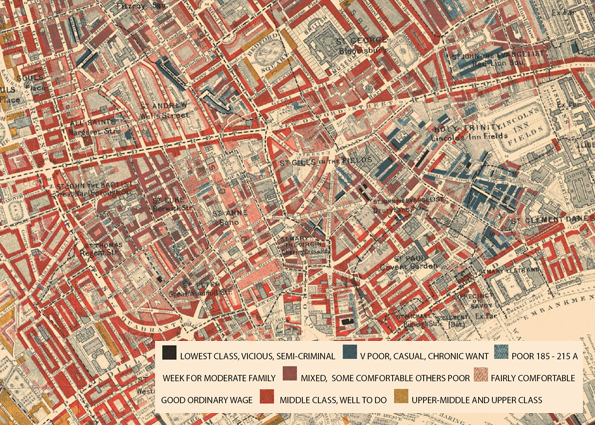
\includegraphics[width=.95\linewidth]{BoothLondonMap.jpg}}
\end{picture}
\end{frame}

\begin{frame}{History}
\textbf{W.E.B.\ DuBois}
\begin{picture}(320,350)
\put(0,225){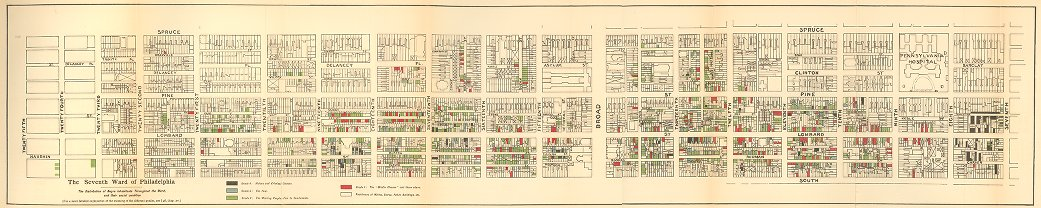
\includegraphics[width=\linewidth]{PhilaNegroDuBoisMapfull.jpg}}
\end{picture}
\end{frame}

\begin{frame}{History}
\textbf{W.E.B.\ DuBois}
\begin{picture}(320,350)
\put(0,225){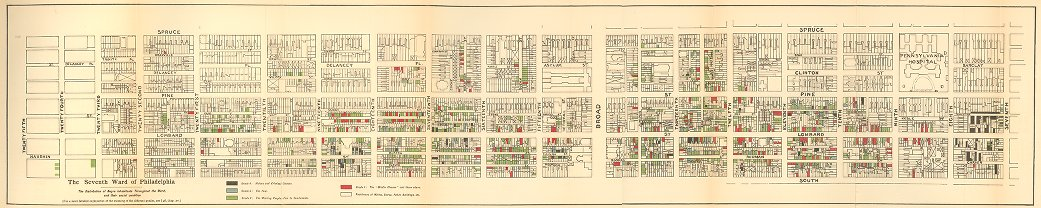
\includegraphics[width=\linewidth]{PhilaNegroDuBoisMapfull.jpg}}
\put(75,200){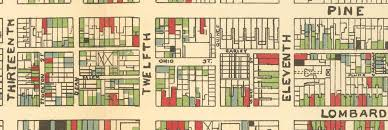
\includegraphics[width=4in]{PhilaNegroDuBoisMapdetail.jpg}}
\end{picture}
\end{frame}

\begin{concept}{Population}
The actual group of people that the survey researcher wants to characterize
\end{concept}

\begin{concept}{Sampling Frame}
The researcher's enumeration of the population
\end{concept}

\begin{frame}{Samples}
Therefore, the sample should \alert{describe the population} and will be \alert{drawn from the sampling frame}
\end{frame}

\begin{frame}{Samples}
\centering
Population
{\LARGE \[\downarrow\]}
Sampling frame
{\LARGE \[\downarrow\]}
Sample
\end{frame}

\begin{frame}{Surveys}
We ask a predefined set of questions to a representative sample of respondents to see how they differ in their answers. 
\end{frame}

{ % all template changes are local to this group.
    \setbeamertemplate{navigation symbols}{}
    \begin{frame}[plain]
	\centering
                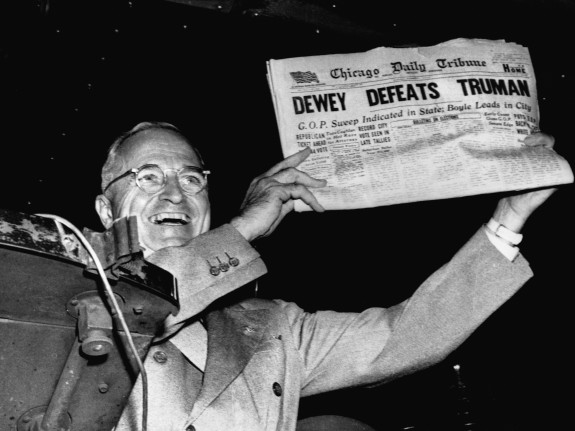
\includegraphics[width=.75\paperwidth]{DeweyDefeatsTruman.jpg}
     \end{frame}
}

\section{Answering Sociological Questions}

\begin{frame}
What are the ontological and epistemological assumptions of survey research? 
\end{frame}

\begin{frame}
What are the advantages and disadvantages of survey methods? 
\end{frame}

\begin{frame}
What types of questions can we answer with survey methods?
\end{frame}

\end{document}


